\documentclass{article}

  % packages
    % basic stuff for rendering math
    \usepackage[letterpaper, top=1in, bottom=1in, left=1in, right=1in]{geometry}
    \usepackage[utf8]{inputenc}
    \usepackage[english]{babel}
    \usepackage{amsmath} 
    \usepackage{amssymb}

    % extra math symbols and utilities
    \usepackage{mathtools}        % for extra stuff like \coloneqq
    \usepackage{mathrsfs}         % for extra stuff like \mathsrc{}
    \usepackage{centernot}        % for the centernot arrow 
    \usepackage{bm}               % for better boldsymbol/mathbf 
    \usepackage{enumitem}         % better control over enumerate, itemize
    \usepackage{hyperref}         % for hypertext linking
    \usepackage{xr-hyper}
    \usepackage{fancyvrb}          % for better verbatim environments
    \usepackage{newverbs}         % for texttt{}
    \usepackage{xcolor}           % for colored text 
    \usepackage{listings}         % to include code
    \usepackage{lstautogobble}    % helper package for code
    \usepackage{parcolumns}       % for side by side columns for two column code
    

    % page layout
    \usepackage{fancyhdr}         % for headers and footers 
    \usepackage{lastpage}         % to include last page number in footer 
    \usepackage{parskip}          % for no indentation and space between paragraphs    
    \usepackage[T1]{fontenc}      % to include \textbackslash
    \usepackage{footnote}
    \usepackage{etoolbox}

    % for custom environments
    \usepackage{tcolorbox}        % for better colored boxes in custom environments
    \tcbuselibrary{breakable}     % to allow tcolorboxes to break across pages

    % figures
    \usepackage{pgfplots}
    \pgfplotsset{compat=1.18}
    \usepackage{float}            % for [H] figure placement
    \usepackage{tikz}
    \usepackage{tikz-cd}
    \usepackage{circuitikz}
    \usetikzlibrary{arrows}
    \usetikzlibrary{positioning}
    \usetikzlibrary{calc}
    \usepackage{graphicx}
    \usepackage{algorithm, algpseudocode}
    \usepackage{caption} 
    \usepackage{subcaption}
    \captionsetup{font=small}

    % for tabular stuff 
    \usepackage{dcolumn}

    \usepackage[nottoc]{tocbibind}
    \pdfsuppresswarningpagegroup=1
    \hfuzz=5.002pt                % ignore overfull hbox badness warnings below this limit

  % New and replaced operators
    \DeclareMathOperator{\Tr}{Tr}
    \DeclareMathOperator{\Sym}{Sym}
    \DeclareMathOperator{\Span}{span}
    \DeclareMathOperator{\std}{std}
    \DeclareMathOperator{\Cov}{Cov}
    \DeclareMathOperator{\Var}{Var}
    \DeclareMathOperator{\Corr}{Corr}
    \DeclareMathOperator{\pos}{pos}
    \DeclareMathOperator*{\argmin}{\arg\!\min}
    \DeclareMathOperator*{\argmax}{\arg\!\max}
    \newcommand{\ket}[1]{\ensuremath{\left|#1\right\rangle}}
    \newcommand{\bra}[1]{\ensuremath{\left\langle#1\right|}}
    \newcommand{\braket}[2]{\langle #1 | #2 \rangle}
    \newcommand{\qed}{\hfill$\blacksquare$}     % I like QED squares to be black

  % Custom Environments
    \newtcolorbox[auto counter, number within=section]{question}[1][]
    {
      colframe = orange!25,
      colback  = orange!10,
      coltitle = orange!20!black,  
      breakable, 
      title = \textbf{Question \thetcbcounter ~(#1)}
    }

    \newtcolorbox[auto counter, number within=section]{exercise}[1][]
    {
      colframe = teal!25,
      colback  = teal!10,
      coltitle = teal!20!black,  
      breakable, 
      title = \textbf{Exercise \thetcbcounter ~(#1)}
    }
    \newtcolorbox[auto counter, number within=section]{solution}[1][]
    {
      colframe = violet!25,
      colback  = violet!10,
      coltitle = violet!20!black,  
      breakable, 
      title = \textbf{Solution \thetcbcounter}
    }
    \newtcolorbox[auto counter, number within=section]{lemma}[1][]
    {
      colframe = red!25,
      colback  = red!10,
      coltitle = red!20!black,  
      breakable, 
      title = \textbf{Lemma \thetcbcounter ~(#1)}
    }
    \newtcolorbox[auto counter, number within=section]{theorem}[1][]
    {
      colframe = red!25,
      colback  = red!10,
      coltitle = red!20!black,  
      breakable, 
      title = \textbf{Theorem \thetcbcounter ~(#1)}
    } 
    \newtcolorbox[auto counter, number within=section]{corollary}[1][]
    {
      colframe = red!25,
      colback  = red!10,
      coltitle = red!20!black,  
      breakable, 
      title = \textbf{Corollary \thetcbcounter ~(#1)}
    } 
    \newtcolorbox[auto counter, number within=section]{proof}[1][]
    {
      colframe = orange!25,
      colback  = orange!10,
      coltitle = orange!20!black,  
      breakable, 
      title = \textbf{Proof. }
    } 
    \newtcolorbox[auto counter, number within=section]{heuristic}[1][]
    {
      colframe = red!25,
      colback  = red!10,
      coltitle = red!20!black,  
      breakable, 
      title = \textbf{Heuristic \thetcbcounter ~(#1)}
    } 
    \newtcolorbox[auto counter, number within=section]{definition}[1][]
    {
      colframe = yellow!25,
      colback  = yellow!10,
      coltitle = yellow!20!black,  
      breakable, 
      title = \textbf{Definition \thetcbcounter ~(#1)}
    } 
    \newtcolorbox[auto counter, number within=section]{example}[1][]
    {
      colframe = blue!25,
      colback  = blue!10,
      coltitle = blue!20!black,  
      breakable, 
      title = \textbf{Example \thetcbcounter ~(#1)}
    } 
    \newtcolorbox[auto counter, number within=section]{code}[1][]
    {
      colframe = green!25,
      colback  = green!10,
      coltitle = green!20!black,  
      breakable, 
      title = \textbf{Code \thetcbcounter ~(#1)}
    } 
    \newtcolorbox[auto counter, number within=section]{algo}[1][]
    {
      colframe = green!25,
      colback  = green!10,
      coltitle = green!20!black,  
      breakable, 
      title = \textbf{Algorithm \thetcbcounter ~(#1)}
    } 

    \definecolor{dkgreen}{rgb}{0,0.6,0}
    \definecolor{gray}{rgb}{0.5,0.5,0.5}
    \definecolor{mauve}{rgb}{0.58,0,0.82}
    \definecolor{darkblue}{rgb}{0,0,139}
    \definecolor{lightgray}{gray}{0.93}
    \renewcommand{\algorithmiccomment}[1]{\hfill$\triangleright$\textcolor{blue}{#1}}

    % default options for listings (for code)
    \lstset{
      autogobble,
      frame=ltbr,
      language=Python,
      aboveskip=3mm,
      belowskip=3mm,
      showstringspaces=false,
      columns=fullflexible,
      keepspaces=true,
      basicstyle={\small\ttfamily},
      numbers=left,
      firstnumber=1,                        % start line number at 1
      numberstyle=\tiny\color{gray},
      keywordstyle=\color{blue},
      commentstyle=\color{dkgreen},
      stringstyle=\color{mauve},
      backgroundcolor=\color{lightgray}, 
      breaklines=true,                      % break lines
      breakatwhitespace=true,
      tabsize=3, 
      xleftmargin=2em, 
      framexleftmargin=1.5em, 
      stepnumber=1
    }

  % Page style
    \pagestyle{fancy}
    \fancyhead[L]{}
    \fancyhead[C]{Muchang Bahng}
    \fancyhead[R]{Spring 2025} 
    \fancyfoot[C]{\thepage / \pageref{LastPage}}
    \renewcommand{\footrulewidth}{0.4pt}          % the footer line should be 0.4pt wide
    \renewcommand{\thispagestyle}[1]{}  % needed to include headers in title page

  % commands 
    \newcommand{\colorwheel}[6]{%
      % #1, #2, #3 = three primary colors (red, yellow, blue)
      % #4, #5, #6 = three secondary colors (orange, green, violet)
      \begin{tikzpicture}[scale=0.8]
        \def\radius{2}
        
        % Complete 12-color wheel (counterclockwise from top)
        \fill[#4!80!#2] (0,0) -- (375:\radius) arc (375:345:\radius) -- cycle;   % Yellow-Orange tertiary
        \fill[#2] (0,0) -- (345:\radius) arc (345:315:\radius) -- cycle;         % Yellow primary
        \fill[#2!80!#5] (0,0) -- (315:\radius) arc (315:285:\radius) -- cycle;   % Yellow-Green tertiary
        \fill[#5] (0,0) -- (285:\radius) arc (285:255:\radius) -- cycle;         % Green secondary
        \fill[#5!80!#3] (0,0) -- (255:\radius) arc (255:225:\radius) -- cycle;   % Blue-Green tertiary
        \fill[#3] (0,0) -- (225:\radius) arc (225:195:\radius) -- cycle;         % Blue primary
        \fill[#3!80!#6] (0,0) -- (195:\radius) arc (195:165:\radius) -- cycle;   % Blue-Violet tertiary
        \fill[#6] (0,0) -- (165:\radius) arc (165:135:\radius) -- cycle;         % Violet secondary
        \fill[#6!80!#1] (0,0) -- (135:\radius) arc (135:105:\radius) -- cycle;   % Red-Violet tertiary
        \fill[#1] (0,0) -- (105:\radius) arc (105:75:\radius) -- cycle;          % Red primary
        \fill[#1!80!#4] (0,0) -- (75:\radius) arc (75:45:\radius) -- cycle;     % Red-Orange tertiary
        \fill[#4] (0,0) -- (45:\radius) arc (45:15:\radius) -- cycle;           % Orange secondary
        
        % Draw the outer circle and sector lines
        \draw[thick, black] (0,0) circle (\radius);
        \foreach \angle in {15, 45, 75, 105, 135, 165, 195, 225, 255, 285, 315, 345} {
          \draw[thick, black] (0,0) -- (\angle:\radius);
        }
        
        % Inner white circle
        \fill[white] (0,0) circle (0.8);
        \draw[thick, black] (0,0) circle (0.8);

        % Add dotted lines through primary colors
        \draw[dotted, thick, black] (90:2.5) -- (270:2.5);     % Through red primary (top to bottom)
        \draw[dotted, thick, black] (330:2.5) -- (150:2.5);    % Through yellow primary (upper left to lower right)
        \draw[dotted, thick, black] (210:2.5) -- (30:2.5);     % Through blue primary (lower left to upper right)
      \end{tikzpicture}
    }

  % external documents 
  %  \externaldocument[place-]{../Machine_Learning/paper}[../Machine_Learning/paper.pdf] 

\begin{document}

\title{Color Theory}
\author{Muchang Bahng}
\date{Fall 2025}

\maketitle
\tableofcontents
\pagebreak

This covers computability theory, complexity theory, and automata theory. 
Alphabet. Boolean logic


\section{Hues} 

  Another way to represent this is with color wheels, which is much simpler and gives artists a starting point to test colors. 

  \begin{definition}[Color Wheel]
    A \textbf{color wheel} is a visual diagram derived from a set of three primary colors.   

    \begin{figure}[H]
      \centering
      \begin{subfigure}[b]{0.32\textwidth}
        \centering
        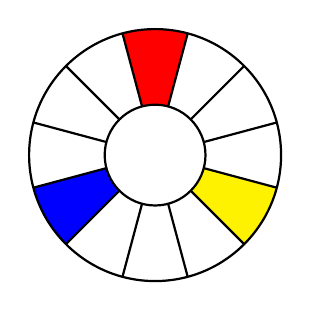
\begin{tikzpicture}[scale=0.8]
          \def\radius{2}
          
          % Complete 12-color wheel (flipped across vertical axis)
          \fill[orange!80!yellow] (0,0) -- (345:\radius) arc (345:375:\radius) -- cycle; % Yellow-Orange
          \fill[yellow] (0,0) -- (345:\radius) arc (345:315:\radius) -- cycle;         % Yellow
          \fill[lime] (0,0) -- (315:\radius) arc (315:285:\radius) -- cycle;           % Yellow-Green
          \fill[green] (0,0) -- (285:\radius) arc (285:255:\radius) -- cycle;          % Green
          \fill[teal] (0,0) -- (255:\radius) arc (255:225:\radius) -- cycle;           % Blue-Green
          \fill[blue] (0,0) -- (225:\radius) arc (225:195:\radius) -- cycle;           % Blue
          \fill[blue!50!magenta] (0,0) -- (195:\radius) arc (195:165:\radius) -- cycle; % Blue-Violet
          \fill[magenta] (0,0) -- (165:\radius) arc (165:135:\radius) -- cycle;        % Violet
          \fill[red!50!magenta] (0,0) -- (135:\radius) arc (135:105:\radius) -- cycle; % Red-Violet
          \fill[red] (0,0) -- (105:\radius) arc (105:75:\radius) -- cycle;              % Red
          \fill[red!50!orange] (0,0) -- (75:\radius) arc (75:45:\radius) -- cycle;     % Red-Orange
          \fill[orange] (0,0) -- (45:\radius) arc (45:15:\radius) -- cycle;            % Orange
          % Fill remaining sectors with white (all except 2, 6, 10)
          \foreach \i in {0,1,3,4,5,7,8,9,11} {
            \fill[white] (0,0) -- ({\i*30+15}:\radius) arc ({\i*30+15}:{(\i+1)*30+15}:\radius) -- cycle;
          }
          
          % Draw the outer circle and sector lines
          \draw[thick, black] (0,0) circle (\radius);
          \foreach \angle in {15, 45, 75, 105, 135, 165, 195, 225, 255, 285, 315, 345} {
            \draw[thick, black] (0,0) -- (\angle:\radius);
          }
          
          % Inner white circle
          \fill[white] (0,0) circle (0.8);
          \draw[thick, black] (0,0) circle (0.8);
        \end{tikzpicture}
        \caption{Primary}
        \label{fig:primary-template}
      \end{subfigure}
      \hfill 
      \begin{subfigure}[b]{0.32\textwidth}
        \centering
        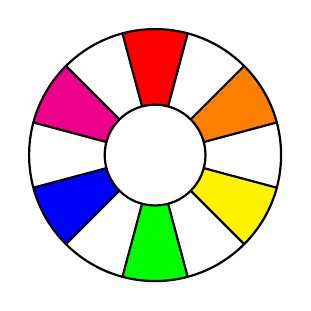
\begin{tikzpicture}[scale=0.8]
          \def\radius{2}
          
          % Complete 12-color wheel (flipped across vertical axis)
          \fill[orange!80!yellow] (0,0) -- (345:\radius) arc (345:375:\radius) -- cycle; % Yellow-Orange
          \fill[yellow] (0,0) -- (345:\radius) arc (345:315:\radius) -- cycle;         % Yellow
          \fill[lime] (0,0) -- (315:\radius) arc (315:285:\radius) -- cycle;           % Yellow-Green
          \fill[green] (0,0) -- (285:\radius) arc (285:255:\radius) -- cycle;          % Green
          \fill[teal] (0,0) -- (255:\radius) arc (255:225:\radius) -- cycle;           % Blue-Green
          \fill[blue] (0,0) -- (225:\radius) arc (225:195:\radius) -- cycle;           % Blue
          \fill[blue!50!magenta] (0,0) -- (195:\radius) arc (195:165:\radius) -- cycle; % Blue-Violet
          \fill[magenta] (0,0) -- (165:\radius) arc (165:135:\radius) -- cycle;        % Violet
          \fill[red!50!magenta] (0,0) -- (135:\radius) arc (135:105:\radius) -- cycle; % Red-Violet
          \fill[red] (0,0) -- (105:\radius) arc (105:75:\radius) -- cycle;              % Red
          \fill[red!50!orange] (0,0) -- (75:\radius) arc (75:45:\radius) -- cycle;     % Red-Orange
          \fill[orange] (0,0) -- (45:\radius) arc (45:15:\radius) -- cycle;            % Orange
          
          
          % Fill remaining sectors with white
          \foreach \i in {1,3,5,7,9,11} {
            \fill[white] (0,0) -- ({\i*30+15}:\radius) arc ({\i*30+15}:{(\i+1)*30+15}:\radius) -- cycle;
          }
          
          % Draw the outer circle and sector lines
          \draw[thick, black] (0,0) circle (\radius);
          \foreach \angle in {15, 45, 75, 105, 135, 165, 195, 225, 255, 285, 315, 345} {
            \draw[thick, black] (0,0) -- (\angle:\radius);
          }
          
          % Inner white circle
          \fill[white] (0,0) circle (0.8);
          \draw[thick, black] (0,0) circle (0.8);
        \end{tikzpicture}
        \caption{Secondary}
        \label{fig:secondary-template}
      \end{subfigure}
      \hfill 
      \begin{subfigure}[b]{0.32\textwidth}
        \centering
        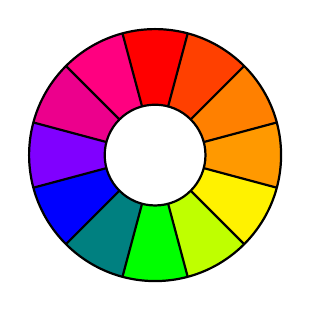
\begin{tikzpicture}[scale=0.8]
          \def\radius{2}
          
          % Complete 12-color wheel (flipped across vertical axis)
          \fill[orange!80!yellow] (0,0) -- (345:\radius) arc (345:375:\radius) -- cycle; % Yellow-Orange
          \fill[yellow] (0,0) -- (345:\radius) arc (345:315:\radius) -- cycle;         % Yellow
          \fill[lime] (0,0) -- (315:\radius) arc (315:285:\radius) -- cycle;           % Yellow-Green
          \fill[green] (0,0) -- (285:\radius) arc (285:255:\radius) -- cycle;          % Green
          \fill[teal] (0,0) -- (255:\radius) arc (255:225:\radius) -- cycle;           % Blue-Green
          \fill[blue] (0,0) -- (225:\radius) arc (225:195:\radius) -- cycle;           % Blue
          \fill[blue!50!magenta] (0,0) -- (195:\radius) arc (195:165:\radius) -- cycle; % Blue-Violet
          \fill[magenta] (0,0) -- (165:\radius) arc (165:135:\radius) -- cycle;        % Violet
          \fill[red!50!magenta] (0,0) -- (135:\radius) arc (135:105:\radius) -- cycle; % Red-Violet
          \fill[red] (0,0) -- (105:\radius) arc (105:75:\radius) -- cycle;              % Red
          \fill[red!50!orange] (0,0) -- (75:\radius) arc (75:45:\radius) -- cycle;     % Red-Orange
          \fill[orange] (0,0) -- (45:\radius) arc (45:15:\radius) -- cycle;            % Orange
          
          % Draw the outer circle and sector lines
          \draw[thick, black] (0,0) circle (\radius);
          \foreach \angle in {15, 45, 75, 105, 135, 165, 195, 225, 255, 285, 315, 345} {
            \draw[thick, black] (0,0) -- (\angle:\radius);
          }
          
          % Inner white circle
          \fill[white] (0,0) circle (0.8);
          \draw[thick, black] (0,0) circle (0.8);
        \end{tikzpicture}
        \caption{Tertiary}
        \label{fig:tertiary-template}
      \end{subfigure}
      \caption{Color wheel progression with primary and secondary colors}
      \label{fig:color-wheel-templates}
    \end{figure}
  \end{definition}

  \begin{example}[Traditional RYB]
    The \textbf{RYB} model is a subtractive color model that uses red, yellow, and blue as the primary colors. 
    \begin{figure}[H]
      \centering 
      \colorwheel{red}{yellow}{blue}{orange}{green}{violet}
      \caption{Traditional artist's color wheel using red, yellow, and blue primaries} 
    \end{figure}
  \end{example}

  \begin{example}[CMY Subtractive]
    The \textbf{CMY} model is a subtractive color model that uses cyan, magenta, and yellow as the primary colors. 
    \begin{figure}[H]
      \centering 
      \colorwheel{cyan}{magenta}{yellow}{blue}{red}{green}
      \caption{Subtractive color model used in printing} 
    \end{figure}
  \end{example}

  \begin{example}[RGB Additive]
    The \textbf{RGB} model is an additive color model that uses red, green, and blue as the primary colors. 
    \begin{figure}[H]
      \centering 
      \colorwheel{red}{green}{blue}{yellow}{cyan}{magenta}
      \caption{Additive color model used in digital displays} 
    \end{figure}
  \end{example} 

\subsection{Contrast}

  The opposite color in the color wheel has the most contrast. 


\subsection{Warm Hues} 

  \begin{example}[Warm Tones]
    \begin{figure}[H]
      \centering 
      \colorwheel{red}{orange}{yellow}{red!70!orange}{yellow!70!red}{orange!70!yellow}
      \caption{Warm-toned color wheel emphasizing reds, oranges, and yellows} 
    \end{figure}
  \end{example}

\subsection{Cool Hues}

  \begin{example}[Cool Tones]
    \begin{figure}[H]
      \centering 
      \colorwheel{blue}{teal}{purple}{cyan}{green}{violet}
      \caption{Cool-toned color wheel emphasizing blues, greens, and purples} 
    \end{figure}
  \end{example}

  \begin{example}[Monochromatic Blue]
    \begin{figure}[H]
      \centering 
      \colorwheel{blue}{blue!70!white}{blue!30!black}{blue!80!cyan}{blue!50!black}{blue!80!purple}
      \caption{Monochromatic color wheel based on blue variations} 
    \end{figure}
  \end{example}

\section{Saturation} 

  \begin{definition}[Tone]
    The \textbf{tone} of a color represents how much gray is in it. 
  \end{definition}

\subsection{Neon Colors}

\section{Brightness}

  \begin{definition}[Brightness]
    The \textbf{brightness} of a color determines how much white or black is in it. 
    \begin{enumerate}
      \item The \textbf{tint} refers to how much white is in it. 
      \item The \textbf{shade} refers to how much black is in it. 
    \end{enumerate}
  \end{definition}

\subsection{Pastel Colors}

\subsection{Muted Colors}



\end{document}
